\documentclass[11pt,a4paper]{article}

%\usepackage[czech]{babel}
\usepackage[utf8]{inputenc}
\usepackage{times}
\usepackage{url}
\usepackage[textwidth=15.2cm,textheight=23cm]{geometry}
\usepackage{xcolor}
\usepackage{color}
\usepackage[unicode, colorlinks,hyperindex,plainpages=false,pdftex]{hyperref}
\usepackage{graphicx}
\usepackage{float}
\usepackage{multirow}

%\usepackage{fancyvrb}
%\DefineVerbatimEnvironment{verbatim}{Verbatim}{}

\usepackage[bf]{caption}

\usepackage[hyperindex,
  plainpages=false,
  pdftex,
  colorlinks,
  pdfborder={0 0 0},
  pdfpagelabels]{hyperref}

\pdfcompresslevel=9

\newcommand{\myincludegraphics}[4]{
  \begin{figure}[!h]
  \centering
  \includegraphics[#1]{#2}
  \caption{#3.} \label{#4}
  \end{figure}
}

% titulní stránka a obsah
\newcommand{\titlepageandcontents}{
  % credits for template go to: Martin Striz
\begin{titlepage}

\vspace*{1cm}

\begin{figure}
  \centering
  
\includegraphics[height=6cm]{images/fit.pdf}
\end{figure}

\vspace*{5mm}

\begin{center}
\begin{Large}
Projekt do předmětu GMU -- Grafické a multimediální procesory
\end{Large}
\end{center}

\vspace*{5mm}

\begin{center}
\begin{Huge}
Komprese/dekomprese JPEG obrázků pomocí 3D akcelerační karty \\
\end{Huge}
\end{center}

\vspace*{1cm}

\begin{center}
\begin{Large}
\today
\end{Large}
\end{center}

\vfill

\begin{flushleft}
\begin{large}
\begin{tabular}{ll}

\bf Řešitelé:\hspace{3mm} 
& Lucie Matušová (\verb_xmatus21@stud.fit.vutbr.cz_) \\
& Jan Wozniak (\verb_xwozni00@stud.fit.vutbr.cz_) \\
& Fakulta Informačních Technologií \\
& Vysoké Učení Technické v~Brně

\end{tabular}
\end{large}
\end{flushleft}

\end{titlepage}

% vim:set ft=tex expandtab enc=utf8:


  \pagestyle{plain}
  \pagenumbering{roman}
  \setcounter{page}{1}
  %\tableofcontents

  \newpage
  \pagestyle{plain}
  \pagenumbering{arabic}
  \setcounter{page}{1}
}

\def\uv#1{\iflanguage{english}{``#1''}%
                              {\quotedblbase #1\textquotedblleft}}%

% vim:set ft=tex expandtab enc=utf8:

\usepackage[czech]{babel}
\usepackage[utf8]{inputenc}
\usepackage{times}
\usepackage{url}
\usepackage[textwidth=15.2cm,textheight=23cm]{geometry}
\usepackage{xcolor}
\usepackage{color}
\usepackage[unicode, colorlinks,hyperindex,plainpages=false,pdftex]{hyperref}
\usepackage{graphicx}
\usepackage{float}
\usepackage{multirow}



\usepackage[bf]{caption}

\pdfcompresslevel=9

\newcommand{\myincludegraphics}[4]{
  \begin{figure}[!h]
  \centering
  \includegraphics[#1]{#2}
  \caption{#3.} \label{#4}
  \end{figure}
}

% titulní stránka a obsah
\newcommand{\titlepageandcontents}{
  % credits for template go to: Martin Striz
\begin{titlepage}

\vspace*{1cm}

\begin{figure}
  \centering
  
\includegraphics[height=6cm]{images/fit.pdf}
\end{figure}

\vspace*{5mm}

\begin{center}
\begin{Large}
Projekt do předmětu GMU -- Grafické a multimediální procesory
\end{Large}
\end{center}

\vspace*{5mm}

\begin{center}
\begin{Huge}
Komprese/dekomprese JPEG obrázků pomocí 3D akcelerační karty \\
\end{Huge}
\end{center}

\vspace*{1cm}

\begin{center}
\begin{Large}
\today
\end{Large}
\end{center}

\vfill

\begin{flushleft}
\begin{large}
\begin{tabular}{ll}

\bf Řešitelé:\hspace{3mm} 
& Lucie Matušová (\verb_xmatus21@stud.fit.vutbr.cz_) \\
& Jan Wozniak (\verb_xwozni00@stud.fit.vutbr.cz_) \\
& Fakulta Informačních Technologií \\
& Vysoké Učení Technické v~Brně

\end{tabular}
\end{large}
\end{flushleft}

\end{titlepage}

% vim:set ft=tex expandtab enc=utf8:


  \pagestyle{plain}
  \pagenumbering{roman}
  \setcounter{page}{1}
  %\tableofcontents

  \newpage
  \pagestyle{plain}
  \pagenumbering{arabic}
  \setcounter{page}{1}
}



\begin{document}
\titlepageandcontents

%---------------------------------------------------------------------------
\section{Zadání}
Úkolem projektu bylo vybrat částí algoritmu při kompresi/dekompresi, které jsou vhodné pro paralelizaci, implementovat
a optimalizovat dané části v OpenCL a nakonec porovant rychlost implementace s CPU. Jelikož implementace JPEG kodéru a
dekodéru je velmi pracnou záležitostí\cite{t81}, rozhodli jsme se výkonnosti jednotlivých částí pipeline implementovat
a měřit zvlášť.

Dále jsou v textu popsány vybrané algoritmy a porovnání paralelních variant na GPU se seriovými, které vykonává CPU.

\section{Použité technologie a zdroje}
\begin{itemize}
\item OpenCL -- pro paralelizaci algoritmů
\item STL kontejnery -- pro usnadnění práce s některými dynamickými typy, tvořen je vektor JPEG markerů
\item Vim -- editor
\item GNU Make -- nástroj pro buildování
\item ostatní zdroje jsou uvedeny mezi citacemi
\end{itemize}

\section{Teoretický rozbor} %asi by bylo vhodne lepe pojmenovat tuto kapitolu
Schéma pipeline pro sekvenční režim JPEG komprese na obrázku \ref{pipeline} obsahuje barevně odlišené bloky, což jsou algoritmy,
které jsme se rozhodli paralelizovat. Mezi jednotlivými bloky jsou uvedeny i datové typy, jaké jsou mezi výstupem
jednoho bloku a vstupem druhého bloku očekávány.

\textit{Převod barevného modelu} je prvním krokem zpracování rastrových dat. Provádíme bezeztrátovou transformaci z barvového prostoru RGB do $YC_bC_r$. Převod jednotlivých složek se provádí podle následujících vzorců:
\begin{eqnarray}
  Y &=& 0,299  R + 0,587  G + 0,114  B\\
  C_b &=& - 0,1687 R - 0,3313 G + 0,5    B + 128\\
  C_r &=&    0,5    R - 0,4187 G - 0,0813 B + 128 
\end{eqnarray}

\textit{Diskrétní kosinová transformace} slouží k převodu obrazu z prostorové domény do frekvenční domény. V normě JPEG
je definováno 6 variant, z nichž nejčastěji používaná Baseline DCT, kterou jsme také v rámci projektu implementovali\cite{mul}. 
Po aplikaci kosinové transformace dostaneme dvě složky koeficientů -- stejnosměrnou (AC) a střídavou (DC). Tyto složky
se dále v algoritmu komprimují zvlášť. Vzorce \ref{dct1}, \ref{dct2} a \ref{dct3} jsou matematickým zápisem DCT,
kde platí, že \textit{N} je pro JPEG blok rovno 8.
\begin{eqnarray}
\lambda_x &=& \left\{ \begin{array}{r@{\quad}c}
    \frac{1}{\sqrt{2}}, & x = 0 \\
    1, & x \neq 0\\ 
\end{array} \right.\label{dct1}\\
g_{k,j}[n,m] &=& \lambda_k \lambda_j \frac{2}{N} cos\left[\frac{k \pi}{N}\left(n+\frac{1}{2}\right)\right] cos\left[\frac{j \pi}{N}\left(m+\frac{1}{2}\right)\right]\label{dct2}\\
c[k,j] &=& \sum^{N-1}_{n=0}{\sum^{N-1}_{m=0}{f[n,m]g_{k,j}[n,m]}}\label{dct3}
\end{eqnarray}


\textit{Kvantizace} je implementována pomocí dvou tabulek, zvlášť pro jasovou složku a chrominescenční složky. Hodnota v 
bloku je nejprve vydělena příslušnou hodnotou v tabulce, zaokrouhlena a poté vynásobena stejnou hodnotou z tabulky.
Pro kvantizaci je definováno několik vhodných tabulek\cite{t81}.

\textit{Huffmanovo kódování} kvantovaných složek probíhá pro stejnosměrné a střídavé koeficienty zvlášť. Před samotným kódováním se tyto složky upraví, aby došlo k redukci výsledného počtu bitů. Nad blokem DC koeficientů spočítáme diferenci, tj. odečteme hodnotu předchozího bloku. Jelikož DC složka odpovídá průměrnému jasu či barvě pixelů v daném bloku a obrázky většinou obsahují souvislé barevné plochy, vniknou takto nízké hodnoty\cite{root}. U AC složek se provádí RLC kódování. Mnoho z nich má totiž nulovou hodnotu, je proto výhodné zapsat sekvence nul efektivně. Výstupem jsou bajty ve tvaru "RRRRSSSS". RRRR je počet nulových koeficientů předcházejicích nenulový koeficient. Pokud je tento počet větší než 15, zapíše se hodnota 0xF0. Pokud jsme na konci a zbývají již samé nuly, zapisuje se 0x00. SSSS značí kategorii hodnoty koeficientu.
Huffmanovo kódování probíhá na základě čtyř tabulek - koeficienty DC a AC, které mohou být pro jasovou složku (Y) nebo barvové složky ($C_b$, $C_r$). U DC složky probíhá tak, že se 11-bitová hodnota diference zakóduje podle jedné z tabulek (Y nebo $C_b$, $C_r$) a za tento kód se přidá samotná hodnota diference ve dvojkovém doplňku. AC koeficienty projdou stejným procesem, akorát jsou pro ně kvůli většímu rozsahu použity rozsáhlejší tabulky.

\begin{figure}[H]
  \centering
  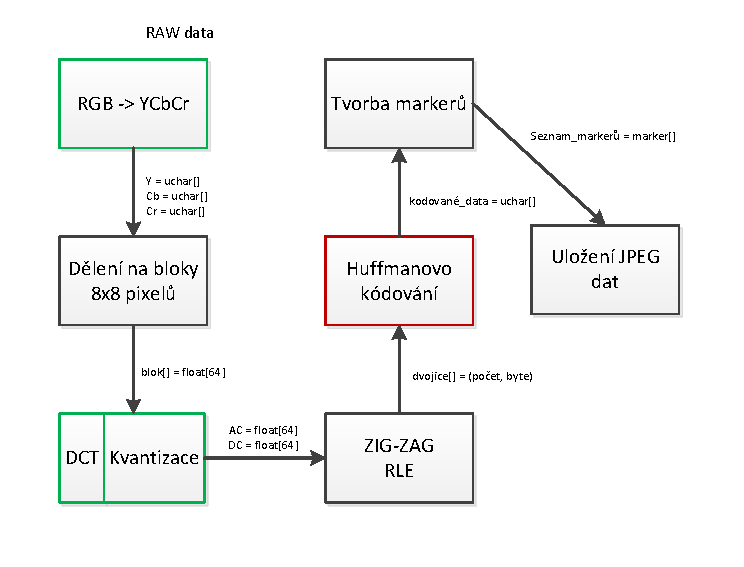
\includegraphics[width=15cm]{pipeline.pdf}
  \caption{Schéma JPEG encode pipeline.}
  \label{pipeline}
\end{figure}

\section{Implementace}
Celý projekt je rozdělen do několika modulů
\begin{itemize}
\item \texttt{cl\_util} -- funkce potřebné pro práci s OpenCL, jednotlivé kernely jsou v souboru \texttt{jpeg.cl}.
\item \texttt{color\_transform} -- funkce pro načtení/uložení obrázku TGA, transformace barevného prostoru a podvzorkování barevných složek 
\item \texttt{dpcm\_rle} -- výpočet diference pro vstupní blok DC koeficientů a rle kódování AC koeficientů dle normy JPEG
\item \texttt{huffman} -- Huffmanovo kódování a kódovací tabulky
\item \texttt{jpeg\_util} -- tvorba a čtení JPEG markerů a další pomocné funkce pro JPEG, které nemají samostaný
modul (zig-zag, kvantizace, DCT ...).
\item \texttt{main} -- funkce \texttt{main} a časová měření algoritmů.
\end{itemize}
\textit{Diskrétní kosinová transformace} je implementována pomocí funkcí

\vspace{0.5em}
\hspace{-1.5em}\texttt{void dct8x8(float* block, float* dct, int* table)} -- sériově\\
\texttt{void dct8x8\_gpu(float* block, float* dst, cl\_mem* table)} -- paralelně
\vspace{0.5em}

kde prvním argumentem jsou data bloku vstupujícího do DCT, druhým argumentem pole pro výstupní AC a DC koeficienty DCT
a třetím argumentem je kvantizační tabulka, neboť v rámci optimalizace jsme sjednotili kvantizaci s DCT.

\textit{Převod barevného modelu} je implementován pomocí dvou funkcí:

\vspace{0.5em}
\hspace{-1.5em}\texttt{void rgb\_to\_ycbcr(pixmap *Y, pixmap *Cb, pixmap *Cr, pixmap *d)} -- sériově\\
\texttt{void ycbcr\_gpu(pixmap* data, unsigned char* dst)} -- paralelně
\vspace{0.5em}

\texttt{pixmap} je struktura obashující rozměry a rastrová data. Do sériového výpočtu vstupují tři pixmapy (Y, $C_b$, $C_r$) pro uložení výsledků a pixmapa s načteným obrázkem. V paralelní implementaci vstupuje pixmapa s obrázkem a druhým argumentem je pole, do kterého se ukládají všechny tři složky. 

\section{Dosažené výsledky}
Výsledkem naší práce je srovnání rychlosti implementací na těchto strojích.
\begin{itemize}
\item Ubuntu -- Core 2 Duo (T7500) 2.20GHz, NVIDIA GeForce 8600M GT
\item Debian -- Core i5 (2500K) 3.3 GHz, NVIDIA GeForce 8800 GTX
\item OS X -- Core i5 (I5-3317U) 1.7 GHz, HD Graphics 4000
\end{itemize}
Hodnoty měření jsou uvedeny v milisekundách, porovnávány jsou paralelní verze a sériové verze algoritmů.
Konverze barevných prostorů byla testována na obrázku 4752x3168 pixelů, DCT je měřena pro jediný blok.

\begin{table}[H]
\begin{center}
\renewcommand{\arraystretch}{1.3} %zvetseni mezer mezi radky v tabulce
\begin{tabular}{|l|cc|cc|cc|}\hline%
\multirow{2}{*}{Algoritmus}&\multicolumn{2}{|c|}{Ubuntu}&\multicolumn{2}{|c|}{Debian}&\multicolumn{2}{|c|}{OS X}\\
          &serial [ms]&paralel [ms]&serial [ms]&paralel [ms]&serial [ms]&paralel [ms]\\\hline%
\texttt{RGB to YCbCr}&1.9269&3.33095    &1.14608&0.874043   &1.24693&1.94597\\
\texttt{YCbCr to RGB}&2.63119&2.99501               &1.63078&0.766993   &1.86396&1.86396\\
\texttt{DCT}         &0.480175&1.13988  &0.320911&0.144005  &0.410795&0.264168\\
\texttt{Inv\_DCT}    &0.487089&1.11485  &0.276089&0.113011  &0.396967&0.203848\\
\hline
\end{tabular}
\renewcommand{\arraystretch}{1} %zvetseni mezer mezi radky v tabulce
\end{center}
\caption{Tabulka srovnání doby výpočtu jednotlivých algoritmů.}
\label{ps_history}
\end{table}

\begin{figure}[H]
  \centering
  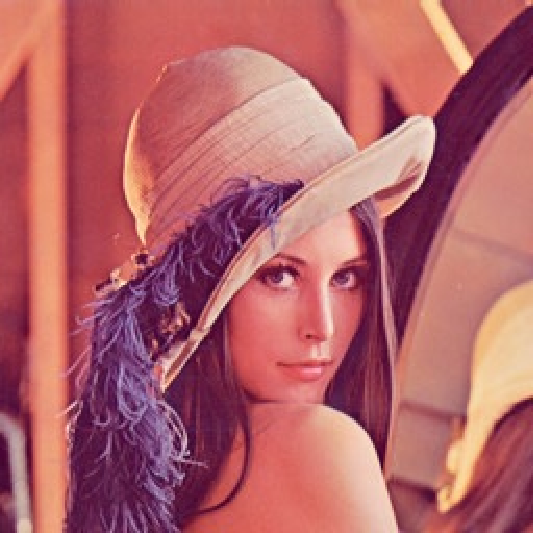
\includegraphics[width=5cm]{sample3.pdf}
  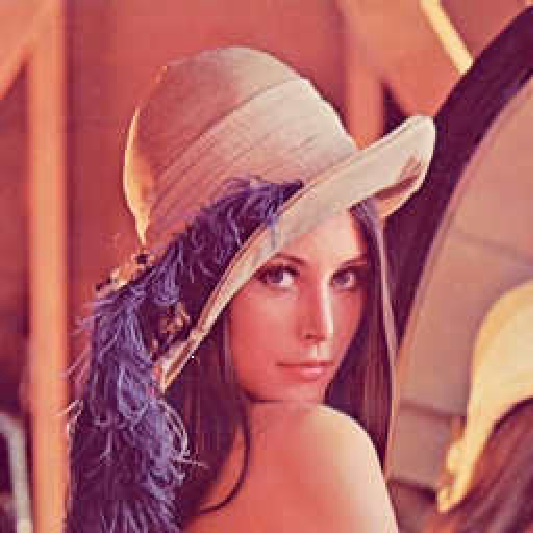
\includegraphics[width=5cm]{sample3_out.pdf}
  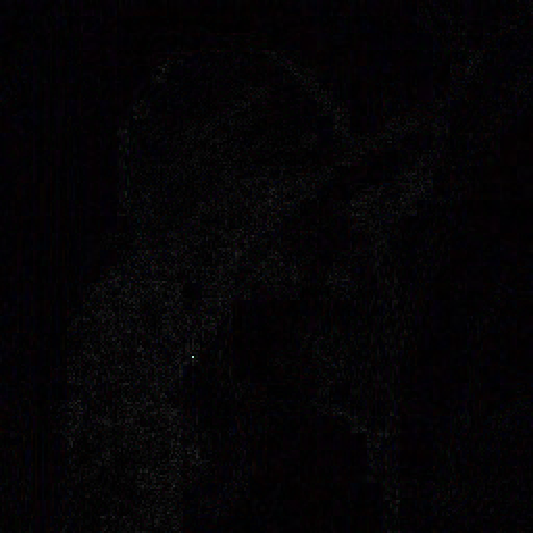
\includegraphics[width=5cm]{sample3_diff.pdf}
  \caption{Srovnání před kompresí a po kompresi.}
  \label{pipeline}
\end{figure}

%---------------------------------------------------------------------------
\section{Rozdělení práce}
\begin{itemize}
\item Lucie Matušová -- převod barevných modelů, extrakce raw dat z TGA formátu, Huffmanovo kódování
\item Jan Wozniak -- DCT, kvantizace, JPEG markery a jeho bloková struktura
\end{itemize}

%---------------------------------------------------------------------------
\section{Co bylo nejpracnější}

Formát JPEG není triviální.  Norma \cite{t81} je složitě napsaná a ostatní zdroje poskytují většinou jen kusé informace. Implementace celé pipeline se nakonec ukázala v daném čase jako nereálná. Od začátku jsme se snažili implementovat všechny části podle doporučení z normy tak, aby bylo možné výsledný soubor dekomprimovat běžným prohlížečem obrázků (např. úpravy koeficientů vstupujících do Huffmanova kódování). Důsledkem byl nedostatek času na paralelizaci Huffmanova kódování.

Komplikace také způsoboval fakt, že jeden z členů týmu nemá na svém počítači podporu OpenCL.

%---------------------------------------------------------------------------
\section{Zkušenosti získané řešením projektu}
Zdokonalili jsme se v programování v OpenCl. Osvojili jsme si práci s jeho paměťovým modelem. Osvěžili jsme si znalosti kódování a důkladně prostudovali JPEG/JFIF. Také jsme si ověřili, že návrh a časový odhad  je na začátku klíčový. Možná by pomohlo na začátku své myšlenky více konzultovat se cvičícími.

%---------------------------------------------------------------------------
\section{Autoevaluace}
\begin{itemize}
\item \textbf{Technický návrh: 60\%} -- původní plán si dával za cíl vytvořit úplný kodér JPEG formátu, což
				není nikterak triviální úloha. Rozhodně přínosnější, než pochopit vnitřní strukturu JPEG
				souboru uloženého na disku by bylo vybrat jen určité algoritmy a důkladněji se zabývat
				optimalizací.
\item \textbf{Programování: 85\%} -- absence rozáhlejších komentářů v některých oblastech může zhoršit čitelnost,
				ale to je jen u triviálních metod/funkcí. Celkově je projekt rozdělen logicky do samostantých
				modulů.
\item \textbf{Vzhled vytvořeného řešení: n/a} -- mělo se jednat o konzolovou aplikaci.
\item \textbf{Využití zdrojů: 90\%} -- přesný popis JPEG formátu poskytuje nejlépe takřka 190 stranová 
				specifikace. Vzhledem k náročnosti tohoto textu bylo ale pro nás nezbytné zpočátku hledat 
				srozumitelnější	informace i jinde.
\item \textbf{Hospodaření s časem: 40\%} -- viz. technický návrh.
\item \textbf{Spolupráce v týmu: 100\%} -- pro verzování kódu jsme použili program Git, práce byla produktivní
				i přes nedotažení původního cíle dokonce.
\item \textbf{Celkový dojem 80\%} -- tím, že je JPEG formát jedním z nejpoužívanějších digitálních obrazových
				formátů, je znalost jeho struktury určitě užitečná pro každého informatika. Rozhodně
				jsme se naučili ocenit práci, kterou udělali jiní programátoři a dříve triviální otevření
				"džejpegu" respektujeme daleko více.
			
\end{itemize}



%
%
% LITERATURA
% ======================
\newpage
{%
    \renewcommand{\refname}{Literatura} % Text nadpisu thebibliography.
    \newcommand{\bi}[4]{\bibitem{#1}\textit{#2.} #3\\{}$<$\url{#4}$>$}%
    \newcommand{\citdatum}[1][2011-10-08]{$[$cit.~{#1}$]$}%
%
\begin{thebibliography}{MM}%
% Vzor: \bi{label}{Název}{Poznámky.}{http://www.adresa.cz/}%
\bi{t81}{Recommendation T.81}{\citdatum[2012-12-10]}
    {http://www.w3.org/Graphics/JPEG/itu-t81.pdf}
\bibitem{mul}{D. Bařina. \textit{Diskrétní kosinová transformace -- prezentace ke cvičení}. \citdatum[2008-12-08].\\
    $<$\url{http://www.fit.vutbr.cz/study/course-l.php.cs?id=8766}$>$}
\bi{wiki}{Wikipedia, the free encyclopedia}{\citdatum[2012-12-10]}
    {http://en.wikipedia.org/}
\bibitem{root}{Pavel Tišnovský. \textit{Ztrátová komprese obrazových dat pomocí JPEG}. ROOT.CZ, 2006, 14.12.}{\citdatum[2012-12-10]}
    $<$\url{http://www.root.cz/clanky/ztratova-komprese-obrazovych-dat-pomoci-jpeg/}    
\end{thebibliography}}

\end{document}
% vim:set ft=tex expandtab enc=utf8:
